\section*{Conclusion}

\begin{frame}{Conclusion}
  \begin{exampleblock}{Fuzzing "bête"}
    \begin{itemize}
      \item{ n'analyse pas du tout le programme pour générer des entrées}
      \item{trouve beaucoup de bugs en pratique}
      \item{exemples : AFL, peach, libfuzzer, ...}
    \end{itemize}
  \end{exampleblock}
  \begin{block}{Fuzzing "intelligent"}
    \begin{itemize}
      \item{peut utiliser de l'exécution symbolique}
      \item{pas très utilisable en pratique}
      \item{exemples : driller, manticore (trailofbits), ...}
    \end{itemize}
  \end{block}
\end{frame}

\begin{frame}{Conclusion}
  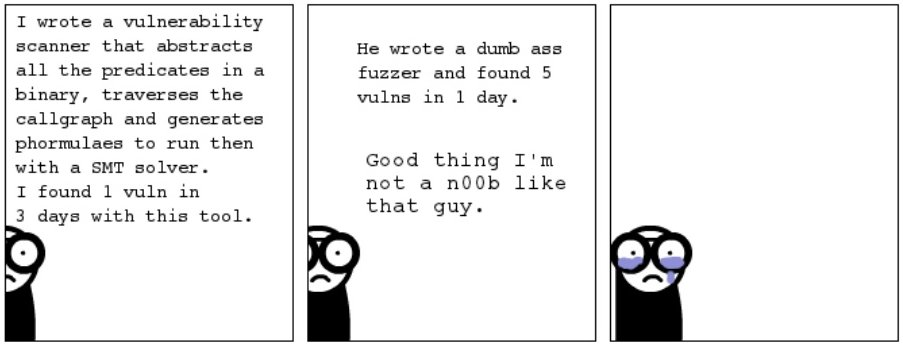
\includegraphics[width=\textwidth]{../medias/comics.png}
\end{frame}
